% #########################################################################
% ##                          FITXER: 7_lstm.tex                         ##
% ##                 Contingut: Capítol de models LSTM                   ##
% #########################################################################

\documentclass[../main.tex]{subfiles}

% ------------------------------------------------------------
% Paquets específics
% ------------------------------------------------------------
\usepackage{paquets_format}
%\usepackage{almutils}

% ------------------------------------------------------------
% Inici del document
% ------------------------------------------------------------
\begin{document}


% ============================================================
% CAPÍTOL: Models LSTM
% ============================================================

\chapter{Modelització amb models LSTM} \label{ch:Models LSTM}

 
\section{Aplicació dels models Long Short-Term Memory (LSTM)}


En la predicció de sèries temporals, s'ha popularitzat l'ús de tècniques basades en \textit{deep learning} per la seva capacitat de captar relacions i patrons de dependència més complexos i no lineals, sobretot a mitjà i llarg termini, difícilment captables pels models estadístics clàssics com serien els ARIMA. Un dels models més utilitzats és les xarxes LSTM (\textit{Long Short-Term Memory}).

En l'aplicació per predicció de series meteorològiques, els models LSTM solen ser comparats amb models clàssics com els ARIMA per avaluar el que pot aportar el \textit{deep learning} com a millora. En general els resultats mostren que les LSTM són particularment útils en series no lineals amb estacionalitats \parencite{lim2021time, de2020comparison}.

Diversos estudis han comparat el rendiment del dos tipus de model aplicats a la predicció de temperatura. \cite{tugal2023analysis} compara els models per a casos de predicció diària d'una regió de Turquia, obtenint resultats més acurats en els models LSTM, segons les mètriques més habituals (RMSE, MSE i MAE). Tanmateix \cite{ozbek2021prediction} també fan aquesta comparació en regions de Turquia, però afinant a escales temporals més petites; en intervals de 10 minuts i de 1 hora, obtenint la mateixa conclusió. No obstant aquesta metodologia no sempre es clarament superior, sinó que probablement està lligada a la situació, tendència de les dades i configuració de paràmetres, ja que en l'estudi de \cite{koccak2023time} els models ARIMA presenten una error lleugerament més baix que les LSTM. Els autor apunten que podria ser a causa del volum baix de dades, i que aquestes presenten una tendència suau de canvi i estacionalitat marcades, per el que en aquest context podria ser millor els models auto-regressius, ja que les xarxes LSTM són més flexibles i capten millor la tendència en presència de sorolls i patrons amb canvis mes bruscos, però que en cas contrari subestimen els valors màxims i sobreestimen els mínims.


\section{Fonament de les RNN i LSTM}

Els models LSTM es basen en l'arquitectura de les \textit{Recurrent Neural Network} (RNN), xarxes neuronals desenvolupades especialment per tractar dades en forma de seqüències, on l'ordre de les observacions és rellevant, a diferència de les altres arquitectures de xarxes neuronals, on les entrades son independents, les RNN incorporen una connexió recursiva que permet transmetre informació d'un pas temporal al següent. Això les fa especialment útils per tasques de predicció temporal, processament llenguatge natural, entre d'altres \parencite{lim2021time}.

Malgrat la seva utilitat, les RNN convencionals presenten una limitació important quan s’apliquen a seqüències llargues: el conegut problema del \textit{vanishing} o \textit{exploding gradient}. Aquest fenomen està relacionat amb el mètode d’entrenament habitual de les xarxes neuronals, basat en la retropropagació (\textit{backpropagation}). Aquesta tècnica ajusta els pesos del model a partir de les derivades de la funció de pèrdua, amb l’objectiu de minimitzar l’error de predicció.

En el cas de les RNN, aquestes derivades es propaguen cap enrere a través de cada pas temporal. Quan les seqüències són molt llargues, aquest procés implica multiplicar moltes derivades entre si. Si aquestes tenen valors menors que 1, el producte es redueix progressivament fins a valors gairebé nuls, fet que impedeix actualitzar els pesos de les primeres etapes: és el que es coneix com a \textit{vanishing gradient}. En canvi, si les derivades són majors que 1, el valor del gradient pot créixer exponencialment, provocant canvis inestables en els pesos ,el que s’anomena \textit{exploding gradient}. En ambdós casos, el resultat és que la xarxa perd la capacitat d’aprendre patrons que depenen de contextos temporals llargs \cite{lim2021time,de2020comparison}.

Per solucionar aquest problema, es van desenvolupar les arquitectura LSTM, que afegeixen un mecanisme específic per regular la memòria. La unitat o neurona LSTM inclou una cèl·lula de memòria i un conjunt de portes que regulen quina informació s’emmagatzema, s’actualitza o s’oblida en cada pas de temps. Aquest disseny les fa especialment robustes per capturar dependències estacionals o cicles llargs, com els que es poden donar en dades meteorològiques \cite{tugal2023analysis}, solucionant així el problema del \textit{vanishing / exploding gradient}.

Cada cèl·lula LSTM conté una estructura interna que li permet conservar informació rellevant durant períodes prolongats Aquesta estructura es basa en un conjunt de mecanismes anomenats \textbf{portes}, que regulen el flux d’informació dins de la cèl·lula, com es transforma i manté la informació en cada pas temporal. 

Els operadors i les funcions que el defineixen de cada cèl·lula LSTM són:


\begin{itemize}
    \item \textbf{Porta d’oblit ($f_t$):} controla quina part de la memòria anterior s’ha d’eliminar.
    \begin{equation}
        f_t = \sigma(W_f \cdot x_t + U_f \cdot h_{t-1} + b_f)
    \end{equation}

    \item \textbf{Porta d’entrada ($i_t$):} regula quina informació nova s’incorpora a la memòria.
    \begin{equation}
        i_t = \sigma(W_i \cdot x_t + U_i \cdot h_{t-1} + b_i)
    \end{equation}

    \item \textbf{Cèl·lula candidata ($\tilde{C}_t$):} genera una proposta d’actualització per a la memòria.
    \begin{equation}
        \tilde{C}_t = \tanh(W_c \cdot x_t + U_c \cdot h_{t-1} + b_c)
    \end{equation}

    \item \textbf{Actualització de la memòria ($C_t$):} combina el que es conserva i el que s’incorpora.
    \begin{equation}
        C_t = f_t \cdot C_{t-1} + i_t \cdot \tilde{C}_t
    \end{equation}

    \item \textbf{Porta de sortida ($o_t$):} decideix quina part de la memòria es propaga com a sortida.
    \begin{equation}
        o_t = \sigma(W_o \cdot x_t + U_o \cdot h_{t-1} + b_o)
    \end{equation}

    \item \textbf{Sortida de la cèl·lula ($h_t$):} resultat final del pas actual, filtrat per la porta de sortida.
    \begin{equation}
        h_t = o_t \cdot \tanh(C_t)
    \end{equation}
\end{itemize}

En aquest conjunt d’equacions, $x_t$ representa l’entrada en el pas temporal $t$, i $h_{t-1}$ és la sortida (o estat ocult) del pas anterior. L’estat intern de memòria es denota com $C_t$, i es va actualitzant al llarg del temps en funció de tres mecanismes de control: la porta d’oblit $f_t$, que filtra la memòria anterior $C_{t-1}$; la porta d’entrada $i_t$, que determina quina nova informació $\tilde{C}_t$ s’incorpora; i la porta de sortida $o_t$, que regula quina part de la memòria es propaga com a sortida $h_t$. 

Les matrius $W_*$ i $U_*$ contenen els pesos associats a les entrades i als estats anteriors, respectivament, i $b_*$ són els termes de biaix de cada porta (on $* = f, i, o, c$ segons el cas). Aquest conjunt de components treballa conjuntament per controlar el flux d’informació dins la cèl·lula i facilitar l’aprenentatge de dependències temporals.

Totes aquestes operacions son regulades per les anomenades funcions d'activació $\sigma(\cdot)$ i  $\tanh(\cdot)$. La funció sigmoide $\sigma(\cdot)$ s’utilitza en les portes per limitar la sortida a l’interval $[0, 1]$, el que permet interpretar el seu valor com una fracció de la informació que passa al següent estat. En canvi, la funció tangent hiperbòlica $\tanh(\cdot)$ s’aplica a les actualitzacions internes de la memòria, mantenint els valors dins l’interval $[-1, 1]$ i afavorint així l’estabilitat numèrica durant l’entrenament.

\begin{figure}[H]
    \centering
    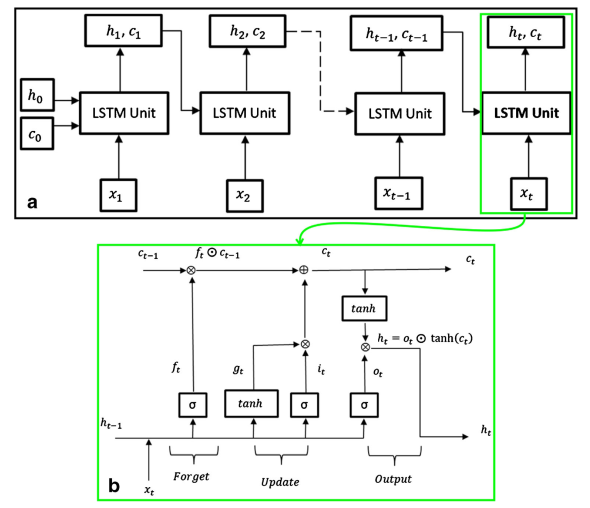
\includegraphics[width=0.5\textwidth]{figures/lstm/concept/2_lstm_cell_NN.png}
    \caption{Arquitectura d’una xarxa LSTM: (a) Xarxa LSTM (b) Flux intern d’informació en una cèl·lula LSTM. 
    Font: \cite{ozbek2021prediction}.}
    \label{fig:lstm_cell_nn}
\end{figure}

A cada pas temporal $t$, la cèl·lula LSTM rep com a entrada $x_t$ i l’estat ocult anterior $h_{t-1}$, (també anomenat estat ocult) i actualitza la seva memòria interna $C_t$ combinant la informació conservada del pas anterior (modulada per la porta d’oblit $f_t$) amb la nova informació rellevant (determinada per la porta d’entrada $i_t$ i la cèl·lula candidata $\tilde{C}_t$). La sortida del pas actual $h_t$ es calcula a partir d’aquest estat intern actualitzat i és filtrada per la porta de sortida $o_t$, per transmetre només la informació rellevant cap a la següent cèl·lula o capa.

Aquest mecanisme flexible (fig \cref{fig:lstm_cell_nn} (b)) permet que cada unitat LSTM aprengui a decidir quina informació recordar, quina oblidar i quina transmetre en funció del context seqüencial de les dades. Gràcies a aquesta capacitat, les xarxes LSTM s’han consolidat com una eina potent per modelitzar dependències temporals complexes.

Una xarxa neuronal LSTM completa està formada per múltiples d’aquestes cèl·lules organitzades seqüencialment i sovint disposades en capes (fig \cref{fig:lstm_cell_nn} (a)) . Cada capa rep com a entrada les sortides temporals de la capa anterior, cosa que permet a la xarxa capturar patrons cada vegada més complexos a diferents nivells de representació temporal.


\section{Estructuració del model}

\subsection{Descripció general del plantejament}

En base als fonaments teòrics de les xarxes LSTM i la naturalesa del nostre problema, s'ha dissenyat un flux de treball i una estructuració d'hiperparàmetres específica amb l'objectiu d'entrenar i confeccionar un model capaç de predir la temperatura horària amb una precisió acceptable.

Aquest flux segueix una estructura modular que permet gestionar de manera flexible i escalable totes les etapes del procés: des del preprocessament de les dades fins a la generació de prediccions. El \textit{pipeline} implementat inclou la càrrega i tractament de les dades, l’escalat dels valors, la generació de seqüències temporals per a l’entrenament, la definició del model LSTM amb diferents configuracions, i finalment, les estratègies de predicció i avaluació.

L’objectiu principal d’aquest esquema és desenvolupar un model robust per a la predicció a curt termini de la temperatura, tot explorant diferents configuracions arquitectòniques i hiperparàmetres que poden afectar el rendiment del model. Així, s’ha establert un conjunt d’experiments per avaluar com canvia la capacitat predictiva del model en funció de la mida de la finestra temporal, el nombre de sortides, la profunditat de la xarxa i altres paràmetres rellevants.


\subsection{Preparació de les dades}

Per a l'entrenament del model s'han escollit el dataset que s'inclou la temperatura horària des del 1-01-2020 fins a 31-12-2024, sense cap interrupció. Aquest es l'interval més recent que no mostra cap interrupció en les dades, tal com s'indica en el \cref{ch:Obtencio i tractament de dades}.

Les dades s'han separat en tres conjunts: 
\begin{itemize}
\item \textit{Test}: per avaluar el rendiment real del model un cop entrenat.  (3 mesos, últims del conjunt)
\item  \textit{Validation}: per monitoritzar l’error. (3 mesos, entre Test i Train)
\item  \textit{Train}: per ajustar els pesos del model. (42 mesos, resta de dades)
\end{itemize}


\begin{figure}[H]
    \centering
    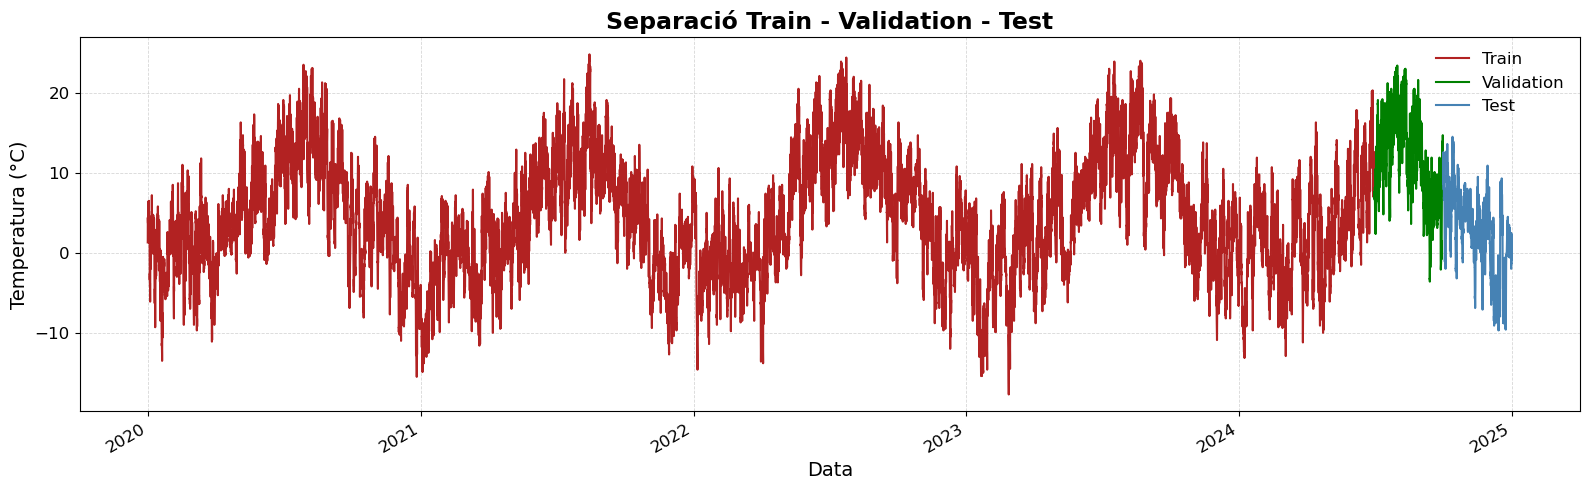
\includegraphics[width=1\linewidth]{figures/lstm/data/data_splits_plot.png}
    \caption{Data Splits (Train, Validation, Test)}
    \label{fig:split_data_plot}
\end{figure}

Amb l’objectiu d’afavorir l’estabilitat numèrica durant l’entrenament i evitar valors descompensats en les funcions d’activació, una pràctica habitual és escalar els valors de les dades en l'interval [0,1], utilitzant una funció escaladora (\cref{eq:scaler}), que converteix el valor mínim el 0, el màxim en 1 i la resta en el rang intermig.
    
\begin{equation}
        x_{scaled} = \dfrac{x - x_{min}}{x_{max} - x_{min}}
        \label{eq:scaler}
    \end{equation}

Aquest procés de transformació es fa només a partir del conjunt de train, i s’extrapola la funció d’escalat als conjunts de validació i test. Aquest detall és important per evitar el fenomen conegut com a \textit{data leaking}, en el que informació del conjunt de test influeixi en el procés d’entrenament del model. Si els valors mínim i màxim s’obtinguessin tenint en compte tot el conjunt de dades, s’estaria introduint informació futura dins la transformació, cosa que falsejaria l’avaluació real del rendiment del model. Finalment, es farà servir la funció inversa per desfer la transformació en els valors predits a la sortida.

Els models LSTM aprenen les relacions a partir de seqüencies de dades per predir la seva continuació. Per això, és necessari transformar la sèrie temporal en un conjunt de seqüències d’entrada i sortida. Aquest procés consisteix a aplicar una finestra mòbil de mida fixa sobre les dades escalades, i generar parelles de mostres $(X, y)$ que permetin a la xarxa aprendre les relacions temporals.

Cada seqüència d’entrada $X$ està formada per un conjunt de valors consecutius de la variable temperatura amb una longitud fixa de \textit{mida de finestra} (paràmetre \texttt{window size}) hores. L’objectiu és que el model, a partir d’aquesta finestra d’informació passada, sigui capaç de predir el valor dels \textit{horitzons de predicció} següents (paràmetre \texttt{num outputs} o \texttt{mostres de sortida}) que segueixen la sèrie de temperatura. Per tant, per a cada seqüència d’entrada, hi ha una seqüència de sortida $y$ amb els valors que es volen predir.


Formalment, el procés de generació de seqüències es pot descriure mitjançant la construcció de parelles $(X_i, y_i)$, on:

\begin{equation}
\begin{aligned}
X_i &= [x_i, x_{i+1}, \dots, x_{i+\text{ws}-1}] \\
y_i &= [x_{i+\text{ws}}, x_{i+\text{ws}+1}, \dots, x_{i+\text{ws}+\text{nout}-1}]
\end{aligned}
\label{eq:seq_generation}
\end{equation}

En aquesta expressió, \( \text{ws} \) és la mida de la finestra d’entrada (\texttt{window size}), i \( \text{nout} \) és el nombre d’horitzons temporals a predir (\texttt{num outputs}). Cada parella $(X_i, y_i)$ representa un exemple d’entrenament, format per una seqüència de valors consecutius i la seva corresponent predicció.

L’estructura final de les dades és un tensor de la forma:
\begin{equation}
\textbf{X}: (n_{\text{mostres}}, \text{window size}, 1)
\quad\quad
\textbf{y}: (n_{\text{mostres}}, \text{num outputs})
\label{eq:formes_dades}
\end{equation}

Aquesta estructura s'aplica als tres conjunts de \textit{Train, Validation i Test}, consolidant els valors de \textit{Windows Size} i \textit{Num Outputs} com els primers hiperparàmetres del model, ja que condicionaran l'entrenament d'aquest.


\subsection{Arquitectura de la xarxa}

L’arquitectura de la xarxa neuronal amb cel·les LSTM es defineix a partir d’un conjunt de paràmetres estructurals i d’entrenament que condicionen tant la capacitat del model com el seu comportament durant l’ajust:

\begin{itemize}
    \item \textbf{Nombre de capes LSTM ($n_{\text{layers}}$)}: determina la profunditat de la xarxa i la seva capacitat per captar patrons temporals complexos.

    \item \textbf{Nombre de neurones per capa ($n_{\text{units}}$)}: indica quantes cel·les LSTM operen en paral·lel dins de cada capa, aportant capacitat del model.

    \item \textbf{Taxa de \textit{dropout}}: fracció de neurones que es desactiven aleatòriament en cada iteració de l'entrenament per reduir el risc de sobre-ajustament.
\end{itemize}


Pel que fa al procés d’entrenament, els principals paràmetres que influeixen en la dinàmica de l’optimització són:

\begin{itemize}
    \item \textbf{Nombre d’èpoques (\textit{Epochs)}}: Nombre de vegades que el model recorre tot el conjunt d’entrenament.

    \item \textbf{Mida del lot (\textit{Batch Size)}}: Nombre de mostres utilitzades en cada actualització dels pesos.

    \item \textbf{Aturada anticipada (\textit{Patience})}:  Nombre d'èpoques sense millora del rendiment, sense disminució de la funció de pèrdua per interrompre l'entrenament i concloure'l a fi d'estalviar recursos computacionals

\end{itemize}

Cal destacar que, tot i que valors més elevats d’aquests paràmetres poden afavorir un millor ajustament, això no sempre es tradueix en un model més robust ni eficient. L’objectiu és trobar un equilibri entre rendiment predictiu, capacitat generalitzadora i eficiència computacional.



\subsection{Resum d'hiperparàmetres del model}

Per tal de dissenyar i ajustar el model LSTM de manera sistemàtica, s’ha definit un conjunt d’hiperparàmetres que controlen el flux de dades, l’arquitectura i el procés d’entrenament. Alguns d’aquests paràmetres s’han mantingut fixos per simplicitat computacional i consistència metodològica, mentre que els altres han estat objecte d’experimentació per analitzar el seu impacte en el model (\cref{tab:resum_hiperparams}).

\begin{table}[H]
    \centering
    \renewcommand{\arraystretch}{1.3}
    \begin{tabular}{lll}
        \toprule
        \textbf{Hiperparàmetre} & \textbf{Valors provats} & \textbf{Tipus} \\
        \midrule
        \texttt{window size}            & [24, 48, 72, 96, 120, 168]& A optimitzar \\
        \texttt{n outputs}                 & [1, 6, 12]                    & A optimitzar \\
        \texttt{n layers}                   & [1, 2, 3]                      & A optimitzar \\
        \texttt{n units}                    & [32, 64, 128]               & A optimitzar \\
        \midrule
        \texttt{dropout}                    &  0.2                           & Fixat \\
        \texttt{batch size}             & 256                           & Fixat \\
        \texttt{epochs}                     & 50                              & Fixat \\
        \texttt{patience}               & 5                                 & Fixat \\
        \bottomrule
    \end{tabular}
    \caption{Resum dels hiperparàmetres considerats en el disseny i entrenament dels models LSTM.}
    \label{tab:resum_hiperparams}
\end{table}


Els valors seleccionats per a cada hiperparàmetre s’han escollit combinant criteris pràctics i referències de la literatura. Els paràmetres com el nombre de capes, de neurones i la mida de finestra s’han variat per analitzar com afecten la capacitat del model de capturar patrons a diferents escales temporals. D’altra banda, paràmetres com  \textit{batch size} o el nombre d’èpoques s’han mantingut constants per reduir la complexitat de l’espai de cerca i facilitar la comparació entre models.

Aquesta selecció permet explorar un conjunt raonable d’arquitectures sense sobrecarregar el cost computacional ni introduir massa variabilitat entre experiments.



\subsection{Estratègies de predicció}

A l’hora d’avaluar el model sobre el conjunt de \textit{test}, es poden aplicar diferents estratègies de predicció, cadascuna amb característiques pròpies que permeten explorar com afecta la forma de generar les prediccions a la qualitat dels resultats obtinguts. Aquestes estratègies es basen en la manera com s’utilitzen les sortides del model per predir múltiples valors consecutius de temperatura.

És important distingir entre els models amb una sola sortida ($n_{\text{outputs}} = 1$) i els que prediuen múltiples valors a la vegada ($n_{\text{outputs}} > 1$). En el primer cas s’han implementat tres estratègies diferenciades: la \textit{Predicció Batch}, la \textit{Predicció Iterativa} i la \textit{Predicció Iterativa amb reinjecció}. En canvi, per als models amb múltiples sortides, només s’ha considerat la \textit{Predicció Batch}, ja que aquests models ja generen els diversos horitzons temporals en una única passada, i les altres estratègies no aporten informació addicional.

\begin{itemize}
    \item \textbf{Predicció \textit{batch}}: el model genera diversos valors futurs d’una sola vegada a partir d’una finestra d’entrada $\mathbf{X}$. Aquesta estratègia és compatible tant amb models de sortida única ($n_{\text{outputs}} = 1$) com múltiple ($n_{\text{outputs}} > 1$), i permet obtenir la seqüència $\mathbf{\hat{y}}$ directament.

    \begin{equation}
        \hat{\mathbf{y}} = \text{Model}(\mathbf{X})
    \end{equation}

    \item \textbf{Predicció iterativa}: en aquest cas el model prediu únicament un pas temporal ($n_{\text{outputs}} = 1$), i les prediccions s’encadenen de forma recursiva: la sortida $\hat{y}_t$ del model es reutilitza com a nova entrada per calcular $\hat{y}_{t+1}$, i així successivament. Aquest enfocament acumula errors amb el temps i tendeix a convergir a un valor constant, però permet explorar horitzons temporals més llargs.

    \begin{equation}
        \hat{y}_{t+1} = \text{Model}([x_{t-n+1}, \dots, x_t]) \Rightarrow \hat{y}_{t+2} = \text{Model}([x_{t-n+2}, \dots, \hat{y}_{t+1}])
    \end{equation}

    \item \textbf{Predicció iterativa amb reinjecció}: aquesta estratègia és similar a l’anterior, però incorpora una actualització periòdica amb les observacions reals. És a dir, cada cert nombre de prediccions (per defecte, cada 5 hores), els valors predit es substitueixen pels valors reals disponible. Això simula un escenari real amb retroalimentació externa i pot ajudar a corregir la deriva del model a llarg termini. A \cref{eq:exemple pred reinjecció} es pot veure un exemple de l'estratègia.
    
\begin{equation}
\begin{aligned}
\hat{y}_{t+1} &= \text{Model}([x_{t-3}, x_{t-2}, x_{t-1}, x_t]) \\
\hat{y}_{t+2} &= \text{Model}([x_{t-2}, x_{t-1}, x_t, \textcolor{blue}{\hat{y}_{t+1}}]) \\
\hat{y}_{t+3} &= \text{Model}([x_{t-1}, x_t, \textcolor{blue}{\hat{y}_{t+1}}, \textcolor{blue}{\hat{y}_{t+2}}]) \\
\hat{y}_{t+4} &= \text{Model}([x_t, \textcolor{blue}{\hat{y}_{t+1}}, \textcolor{blue}{\hat{y}_{t+2}}, \textcolor{blue}{y_{t+3}}]) \\
\hat{y}_{t+5} &= \text{Model}([\textcolor{blue}{\hat{y}_{t+1}}, \textcolor{blue}{\hat{y}_{t+2}}, \textcolor{blue}{y_{t+3}}, \textcolor{blue}{\hat{y}_{t+4}}]) \quad \text{(reinjecció)} \\
\hat{y}_{t+6} &= \text{Model}([\textcolor{red}{x_{t+2}}, \textcolor{red}{x_{t+3}}, \textcolor{red}{x_{t+4}}, \textcolor{red}{x_{t+5}}])
\end{aligned}
\label{eq:exemple pred reinjecció}
\end{equation}

\end{itemize}


\section{Plantejament de models}

Amb l’objectiu d’avaluar el rendiment dels models LSTM en la predicció de temperatura horària, s’ha dissenyat una sèrie d’experiments que permetin analitzar l’efecte dels diferents paràmetres sobre la qualitat de les prediccions. La idea és identificar configuracions que ofereixin un bon equilibri entre precisió, simplicitat i robustesa.

Els experiments s’han dissenyat amb l’objectiu de respondre diverses qüestions pràctiques sobre l’arquitectura i el comportament dels models. Per tal d’estructurar aquesta anàlisi de manera clara i sistemàtica, els experiments s’han agrupat en blocs segons el paràmetre principal que es vol estudiar en cada cas (\cref{tab:config_lstm_models_exp}).

\begin{itemize}
    \item Analitzar com influeix la mida de la finestra d’entrada (\texttt{window\_size}) en la capacitat del model per captar les dinàmiques temporals, combinat amb diverses sortides i profunditats de xarxa.

    \item Comparar models amb sortida única (\texttt{n\_outputs} = 1) i models multioutput de 6 o 12 hores.

    \item Avaluar com afecta la profunditat de la xarxa (\texttt{n\_layers}) i el nombre de neurones per capa (\texttt{n\_units}) al rendiment. 
\end{itemize}

\begin{table}[H]
    \centering
    \renewcommand{\arraystretch}{1.3}
    \small
    \begin{tabular}{lrrrrl}
        \toprule
         \textbf{ID} & \texttt{window\_size} & \texttt{n\_outputs} & \texttt{n\_layers} & \texttt{n\_units} & \textbf{Notes} \\
        \midrule
         BSL   & 24  & 1  & 1 & 32  & Capacitat mínima \\
         \specialrule{1pt}{1pt}{1pt}
         Exp0  & 24  & 1  & 2 & 64  & Model senzill, horitzó curt \\
         Exp1  & 96  & 1  & 3 & 128 & Model potent 1 hora \\
         Exp2  & 96  & 6  & 2 & 64  & Multioutput 6 hores \\
         Exp3  & 96  & 12 & 3 & 128 & Multioutput 12 hores \\
         Exp4  & 168 & 1  & 3 & 64  & Seqüència llarga \\
         Exp5  & 48  & 1  & 1 & 32  & Model lleuger, realista \\
         Exp6  & 120 & 1  & 3 & 64  & Context llarg \\
         \specialrule{1pt}{1pt}{1pt}
         A0 & 96 & 1 & 1 & 64  & Xarxa senzilla \\
         A1 & 96 & 1 & 2 & 64  & Xarxa mitjana \\
         A2 & 96 & 1 & 3 & 64  & Xarxa profunda \\
         \specialrule{1pt}{1pt}{1pt}
         B0 & 96 & 1 & 2 & 32  & Xarxa petita \\
         B1 & 96 & 1 & 2 & 64  & Capacitat intermèdia \\
         B2 & 96 & 1 & 2 & 128 & Xarxa gran \\
         \specialrule{1pt}{1pt}{1pt}
         C0 & 96 & 1 & 1 & 32  & Model lleuger \\
         C1 & 96 & 1 & 1 & 64  & Equilibri senzill \\
         C2 & 96 & 1 & 1 & 128 & Alta capacitat plana \\
        \bottomrule
    \end{tabular}
    \caption{Configuracions experimentals dels models LSTM. S’identifiquen les sèries d’experiments (finals, A, B i C) i les variants de paràmetres més rellevants.}
    \label{tab:config_lstm_models_exp}
\end{table}



\section{Resultats}

En la \cref{tab:resultats_models_lstm}  es poden veure les mètriques per avaluar els diferents models LSTM entrenats tant amb l’estratègia de predicció \textit{batch} (directa) com amb la de \textit{reinjecció} (recursiva corregida). En general, en els models amb una sola sortida, la predicció \textit{batch} sol donar molt bons resultats, amb RMSE < 1. Això és esperable, ja que el model disposa de tota la seqüència passada per predir només una hora endavant ,la següent dada, cosa que té poc valor pràctic en el context real del problema. Per això, resulta més rellevant avaluar el rendiment en l’escenari de \textit{reinjecció}, on les prediccions del model es van reutilitzant i acumulant, simulant un escenari real.

S’observa que el model base (\texttt{BSL}) presenta un rendiment força limitat, amb valors d’error relativament alts, especialment en la predicció amb reinjecció, on l’error creix de forma important. Aquest model, amb una arquitectura mínima, serveix com a punt de referència per quantificar les millores obtingudes la resta de models, establint una mena de llindar mínim de predicció.
\begin{table}[H]
    \centering
    \small
    \renewcommand{\arraystretch}{1.3}
    \setlength{\tabcolsep}{6pt}
    \begin{tabular}{l|ccc|ccc}
        \toprule
        \textbf{ID} & \multicolumn{3}{c|}{\textbf{Predicció batch}} & \multicolumn{3}{c}{\textbf{Predicció reinjecció}} \\
        & \textbf{RMSE} & \textbf{MSE} & \textbf{MAE} & \textbf{RMSE} & \textbf{MSE} & \textbf{MAE} \\
        \midrule
        BSL     & 0.99267 & 0.8588 & 0.7212 & 2.3256 & 5.4085 & 1.7917 \\
        \specialrule{1pt}{1pt}{1pt}
        Exp0    & 0.7883 & 0.6214 & 0.542 & 1.6214 & 2.6289 & 1.1492 \\
        Exp1    & 0.8358 & 0.6986 & 0.6026 & 1.7257 & 2.9779 & 1.2662 \\
        Exp2    & 1.7069 & 2.9136 & 1.2301 & - & - & - \\
        Exp3    & 2.8366 & 8.0462 & 2.1109 & - & - & - \\
        Exp4    & 0.8239 & 0.6788 & 0.5941 & 1.8156 & 3.2965 & 1.3427 \\
        Exp5    & 0.8696 & 0.7563 & 0.6538 & 2.0572 & 4.2319 & 1.5592 \\
        \textbf{Exp6}    & \textbf{0.7685} & \textbf{0.5906} & \textbf{0.5166} & \textbf{1.52} & \textbf{2.3104} & \textbf{1.0436} \\
        \specialrule{1pt}{1pt}{1pt}
        A0      & 0.8468 & 0.7171 & 0.6298 & 2.047 & 4.1901 & 1.5608 \\
        A1      & 0.8003 & 0.6450 & 0.5611 & 1.6095 & 2.5906 & 1.1565 \\
        A2      & 0.7955 & 0.6328 & 0.5488 & 1.5005 & 2.2516 & 1.0535 \\
        \specialrule{1pt}{1pt}{1pt}
        B0      & 0.847 & 0.7175 & 0.6395 & 1.9343 & 3.7415 & 1.4798 \\
        B1      & 0.8003 & 0.6405 & 0.5611 & 1.6095 & 2.5906 & 1.1565 \\
        B2      & 0.7994 & 0.6391 & 0.5965 & 1.6566 & 2.7443 & 1.1955 \\
        \specialrule{1pt}{1pt}{1pt}
        C0      & 0.9597 & 0.9211 & 0.747 & 2.1274 & 4.9169 & 1.7294 \\
        C1      & 0.8443 & 0.7128 & 0.6268 & 1.9396 & 3.7619 & 1.4767 \\
        C2      & 0.7538 & 0.5683 & 0.5220 & 1.5440 & 2.3840 & 1.0966 \\
        \bottomrule
    \end{tabular}
    \caption{Resultats dels models LSTM: mètriques de predicció per a batch i reinjecció}
    \label{tab:resultats_models_lstm}
\end{table}


Els models de la sèrie \texttt{Exp} representen una exploració diversa de configuracions: des de arquitectures lleugeres (com \texttt{Exp0} i \texttt{Exp5}) fins a models profunds i amb múltiples sortides (\texttt{Exp2} i \texttt{Exp3}). Es pot destacar que els models amb una sola sortida (\texttt{n\_outputs = 1}) i més profunditat (\texttt{Exp1}, \texttt{Exp4}, \texttt{Exp6}) milloren considerablement el rendiment respecte al model base. 

Contràriament, les configuracions amb sortides múltiples (\texttt{Exp2}, \texttt{Exp3}) mostren valors d’error clarament superiors. En aquests casos, tot i que la tendència general de les prediccions sembla seguir la sèrie real, sovint es produeix un desfasament temporal, clarament visible en els gràfics de predicció (\cref{fig:exp3}). Probablement aquest fenomen es causat per una acumulació d'error entre les varies previsions que surten del model, cosa que li dificulten anticipar canvis al anar predint en bloc, de manera que per minimitzar l'error aquest acaba assimilant valors pròxims als anteriors, fent, sense planificar-ho, una estratègia similar a la que duen a terme els models de persistència, cosa que segurament origina el desfasament

Per intentar abordar aquest problema, es va experimentar amb el paràmetre \texttt{lookahead}, desplaçant la finestra d’entrada temporalment per ajudar al model a situar-se millor en el context. Tot i això, els resultats no van mostrar una millora clara, cosa que suggereix que el desfasament no es corregeix només ajustant l’entrada, sinó que pot ser necessari augmentar la capacitat del model o bé incorporar més informació contextual (per exemple, afegir dades sobre el dia i la hora).

El model \texttt{Exp6} (\cref{fig:exp6}), amb finestra llarga, 3 capes, i un nombre de neurones mig (64), ofereix els millors resultats globals amb RMSE de 0.768 en batch i 1.52 amb reinjecció.

Les sèries d’experiments A, B i C exploren de manera sistemàtica l’efecte de la profunditat i la capacitat del model. La Sèrie A es basa en una profunditat de xarxa fixa, on els resultats mostren millora progressiva en les mètriques a mesura que augmenta la profunditat (\cref{fig:a0a2}). L’arquitectura amb 3 capes (\texttt{A2}) presenta els millors resultats dins la sèrie, evidenciant que pot captar patrons mes complexos.
    
Per altra banda, la sèrie B i C es basen en l'extensió de les capes. En cas de la B, igual profunditat (2 capes), es comprova que augmentar les neurones millora lleugerament l’error, tot i que a partir de 64 unitats (model \texttt{B1}) el guany addicional és reduït. En contrapartida, la sèrie C, representa models plans, on es manté la profunditat mínima (1 capa) i es varia la capacitat. Els resultats indiquen que una única capa amb prou neurones (\texttt{C2}) pot obtenir resultats molt competitius, fins i tot comparables amb models més complexos (\cref{fig:c0c2}).

\begin{figure}[H]
    \centering

    % Fila 1
    \begin{subfigure}[b]{0.48\textwidth}
        \centering
        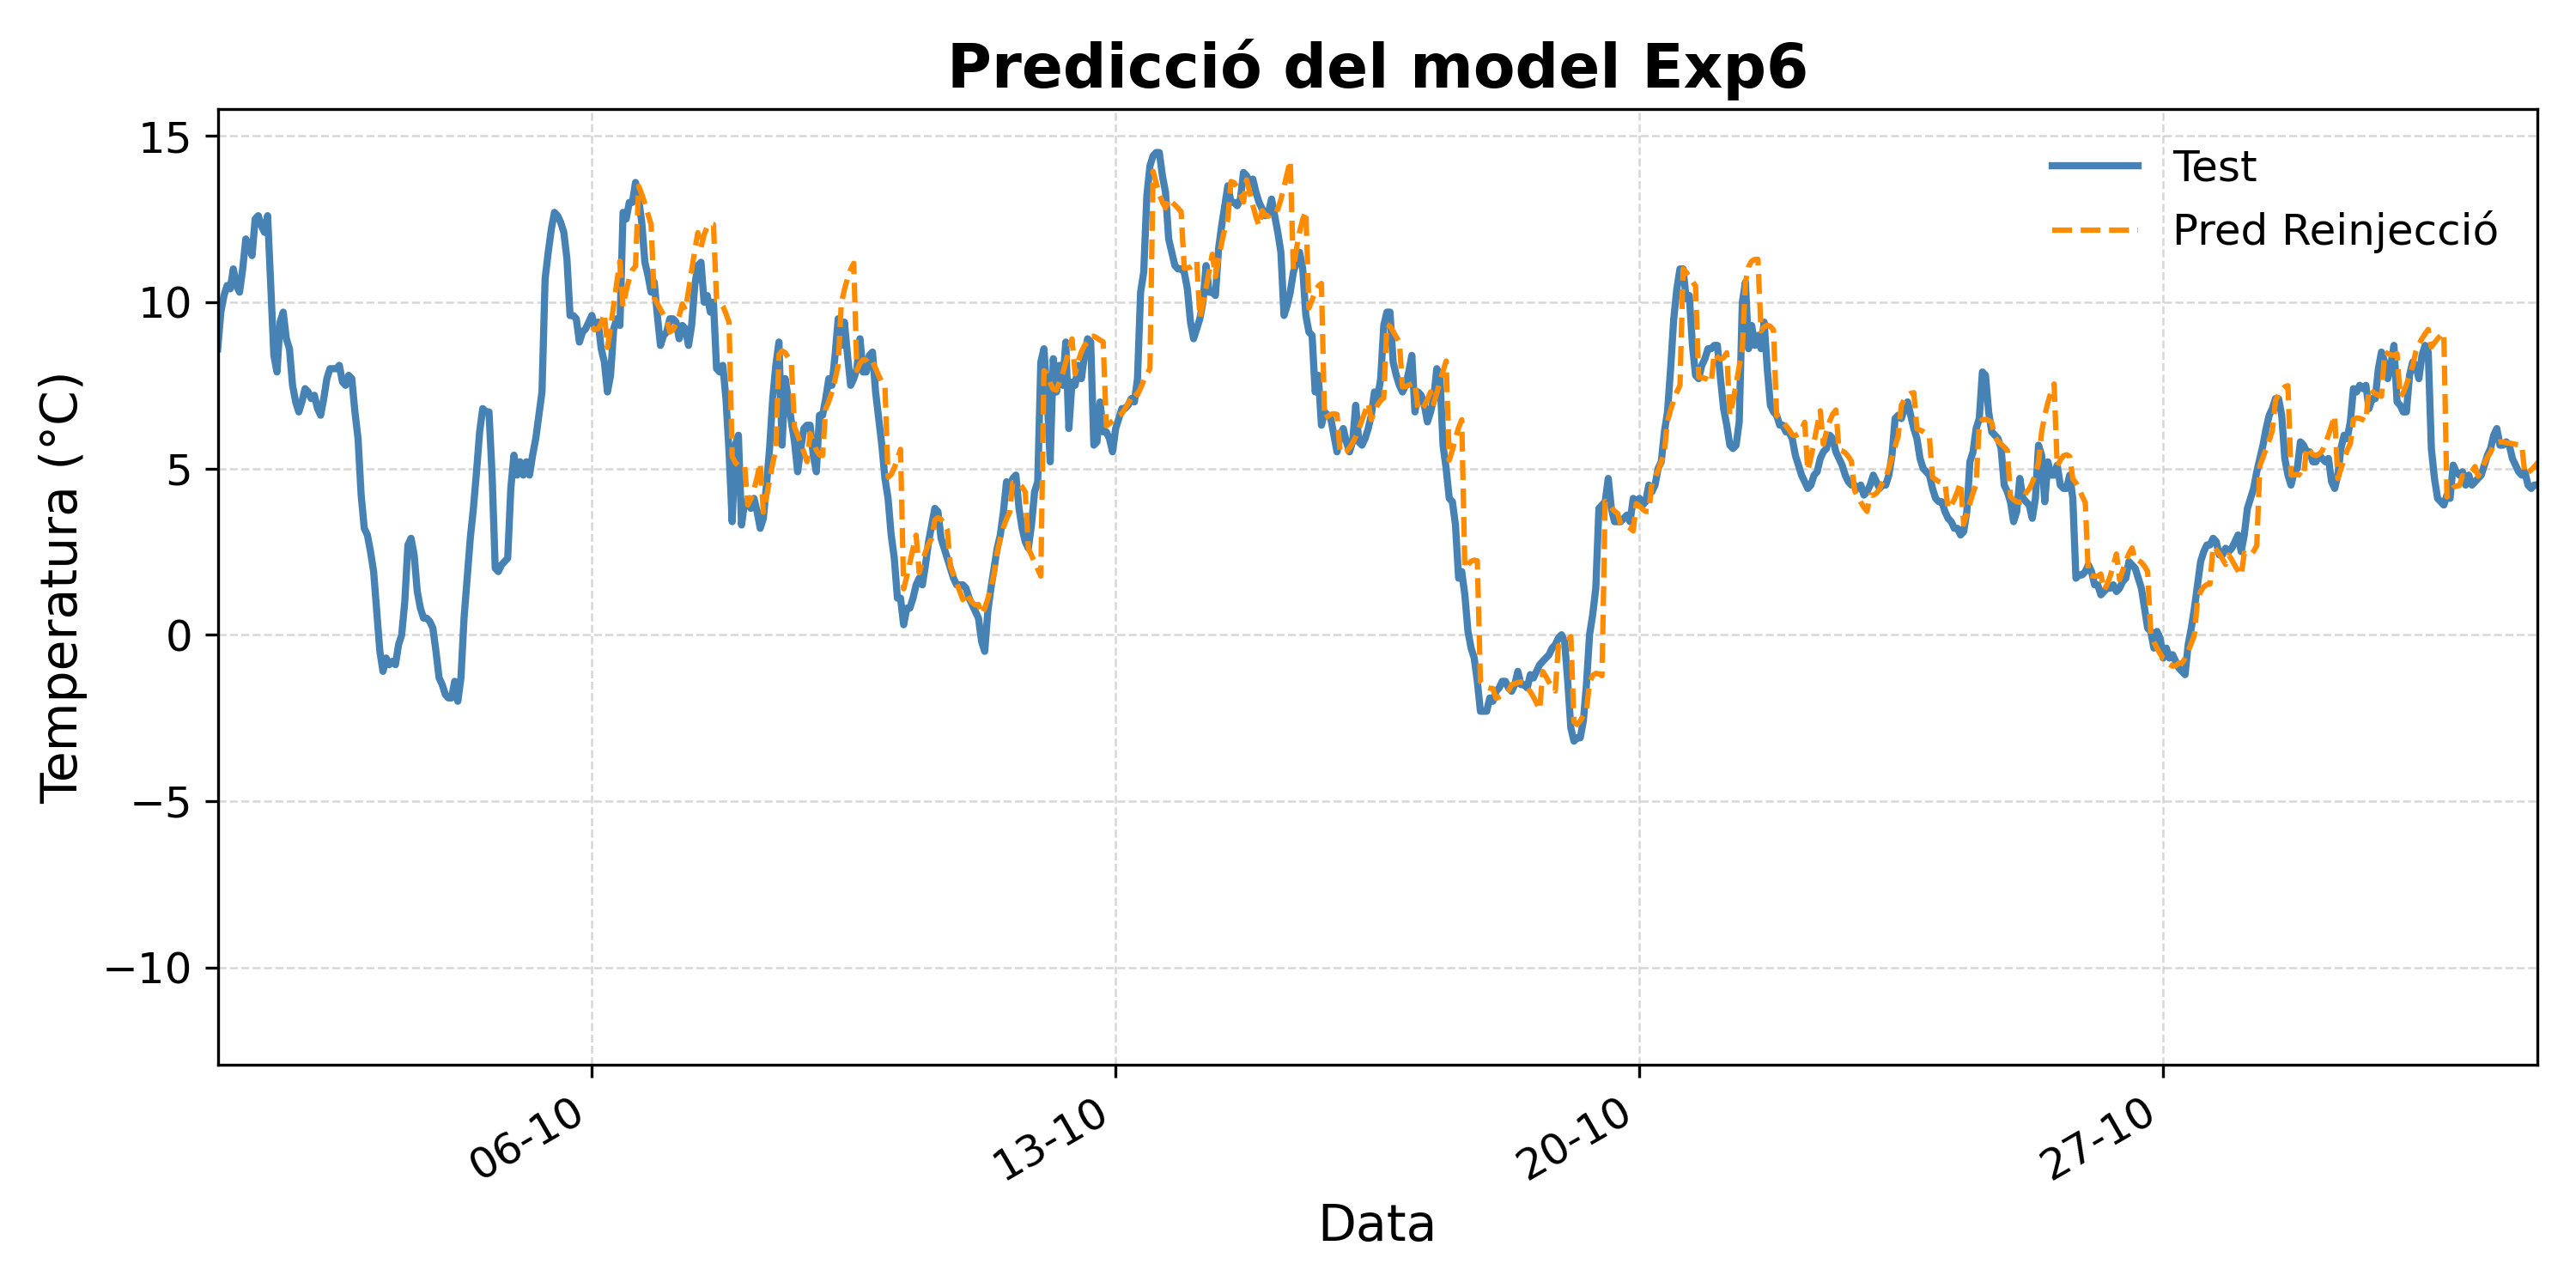
\includegraphics[width=\textwidth]{figures/lstm/results/Exp6_plot_def.png}
        \caption{Model \texttt{Exp6} (reinjecció)}
        \label{fig:exp6}
    \end{subfigure}
    \hfill
    \begin{subfigure}[b]{0.48\textwidth}
        \centering
        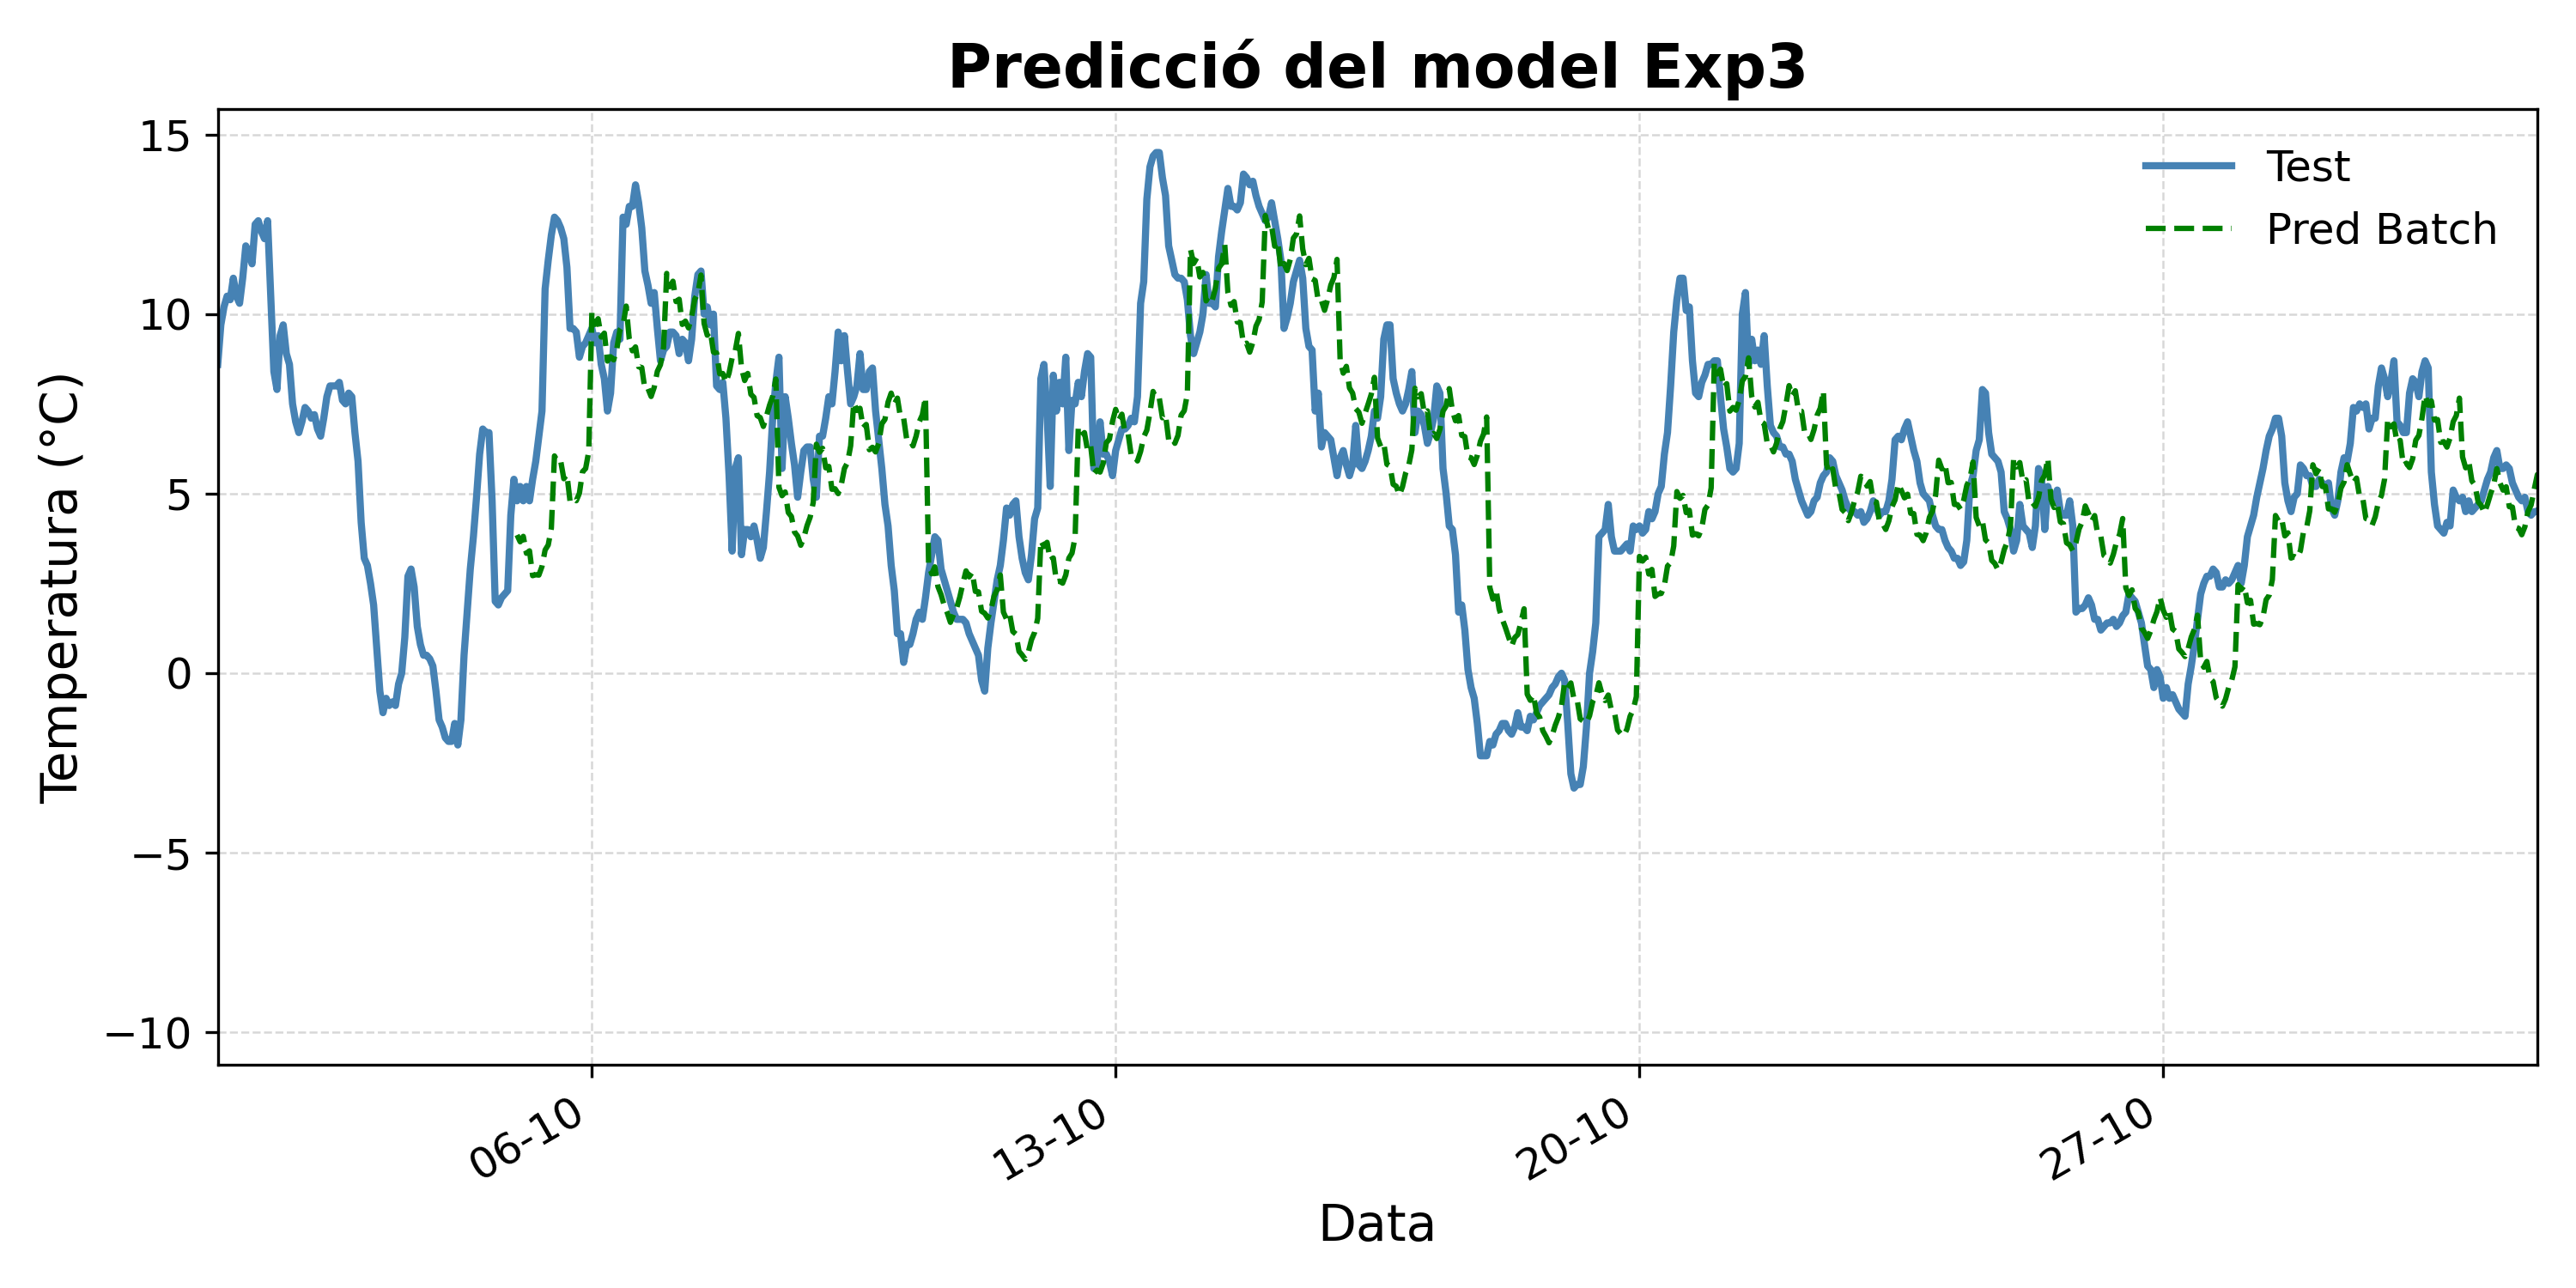
\includegraphics[width=\textwidth]{figures/lstm/results/Exp3_plot_def.png}
        \caption{Model \texttt{Exp3} (predicció \textit{batch})}
        \label{fig:exp3}
    \end{subfigure}

    \vspace{0.5cm}

    % Fila 2
    \begin{subfigure}[b]{0.48\textwidth}
        \centering
        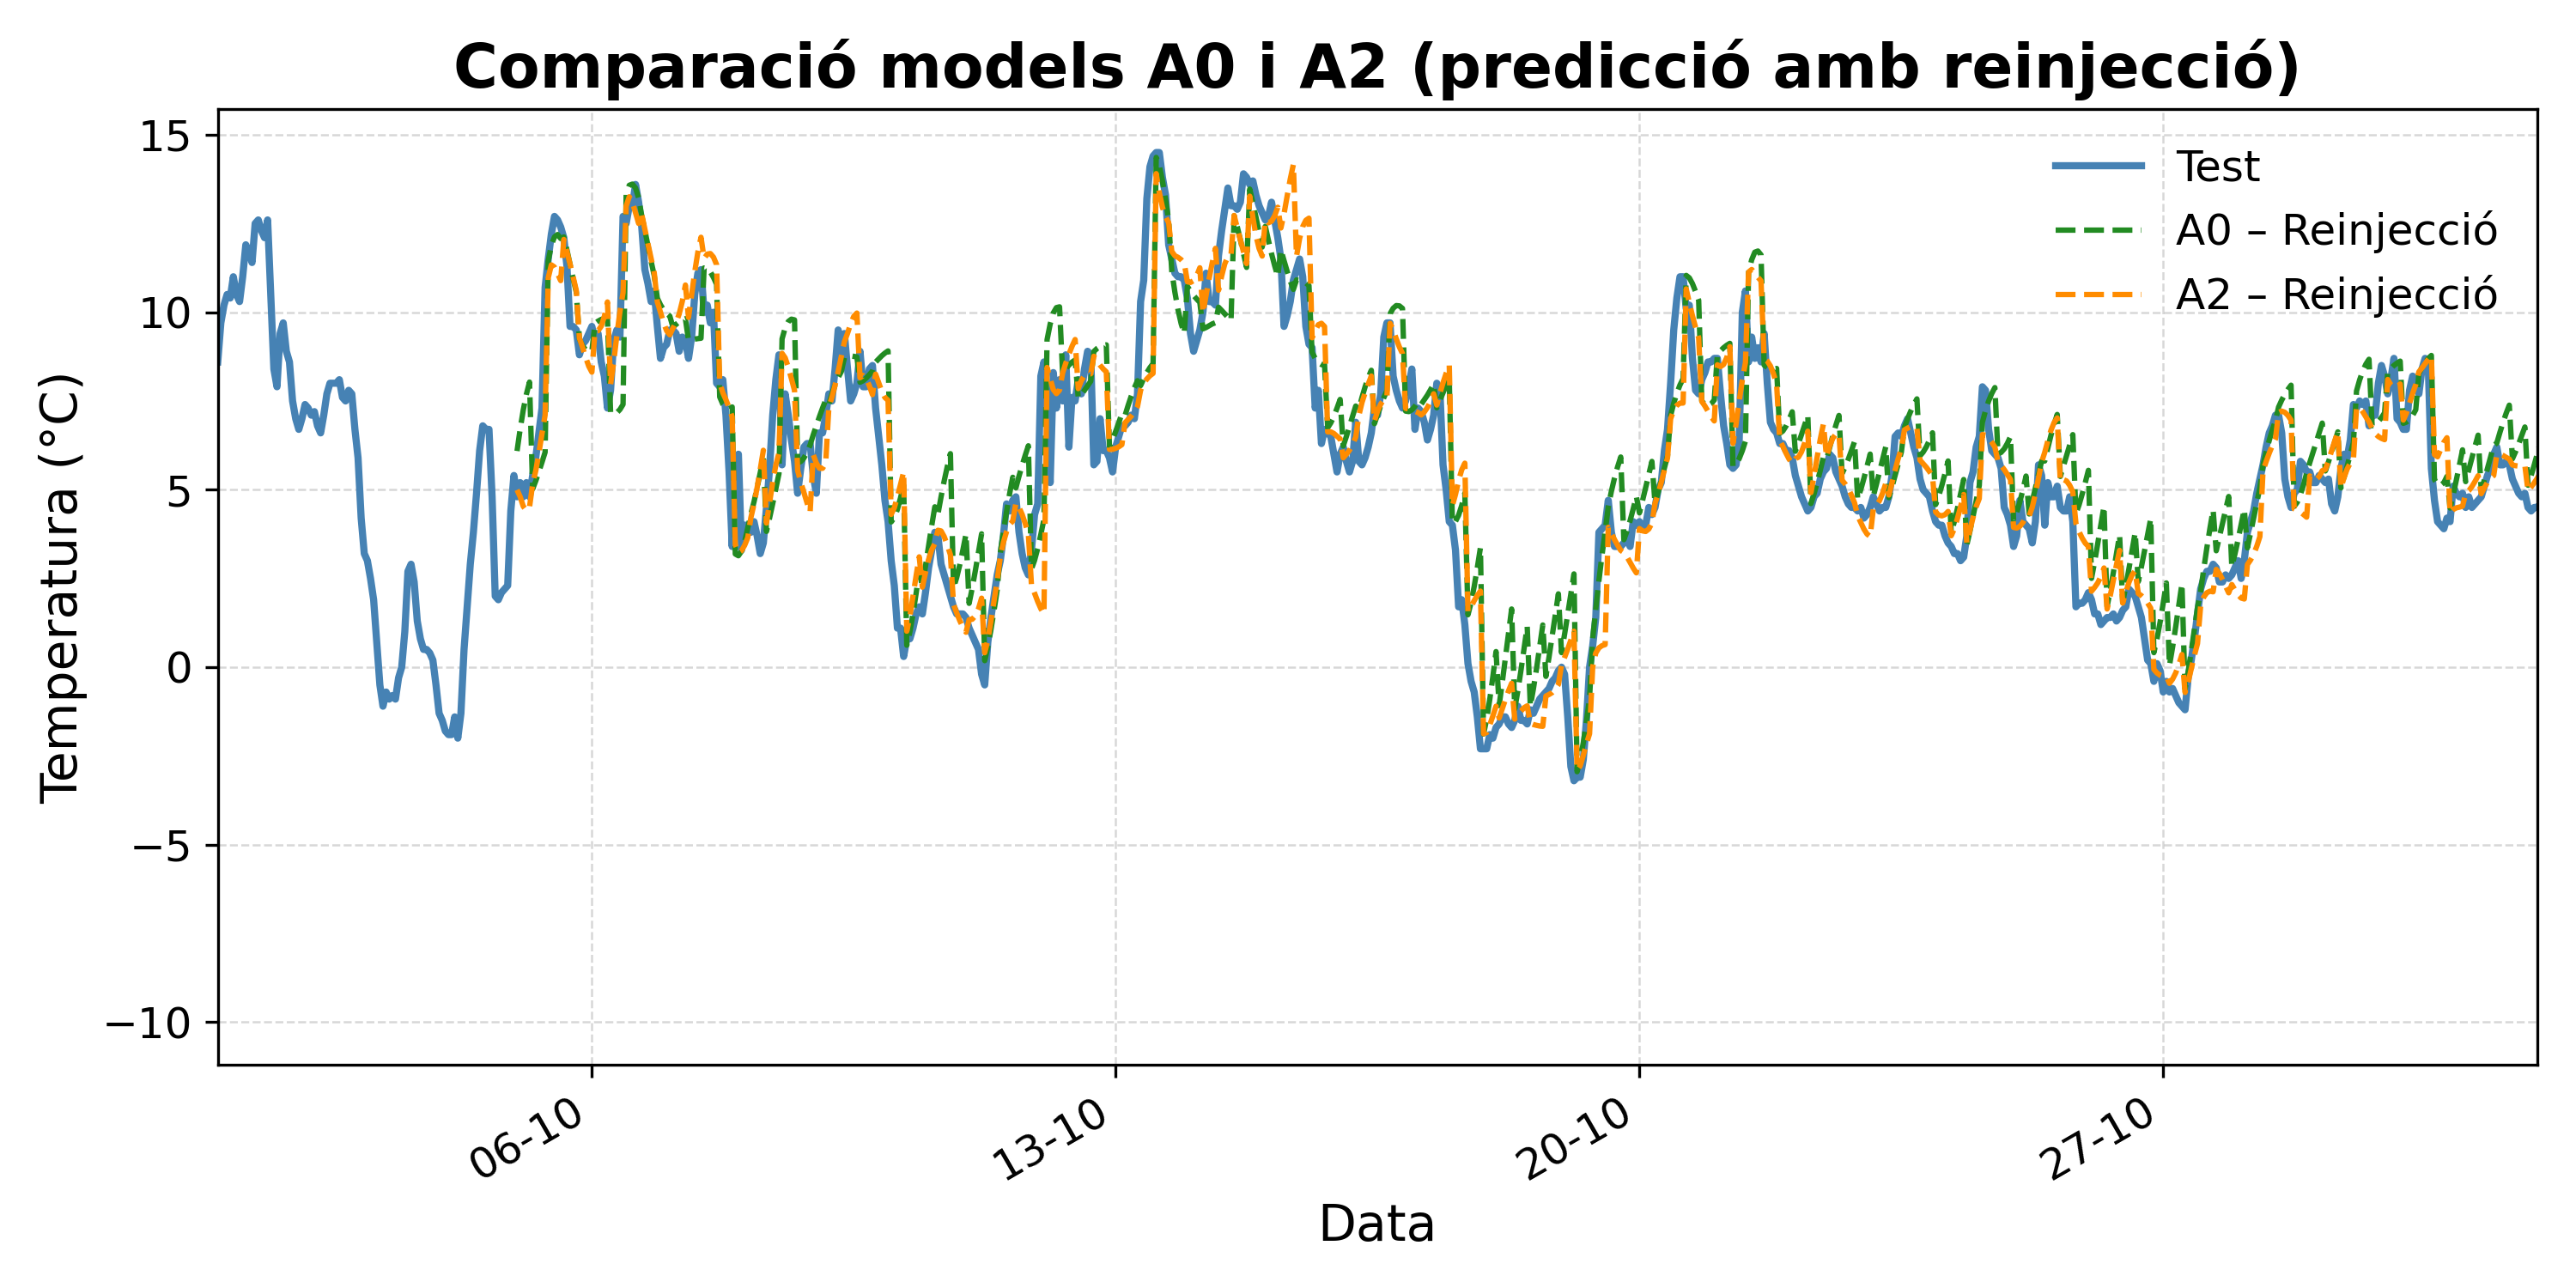
\includegraphics[width=\textwidth]{figures/lstm/results/A0_A2_plot_def.png}
        \caption{Comparació \texttt{A0} vs \texttt{A2} (reinjecció)}
        \label{fig:a0a2}
    \end{subfigure}
    \hfill
    \begin{subfigure}[b]{0.48\textwidth}
        \centering
        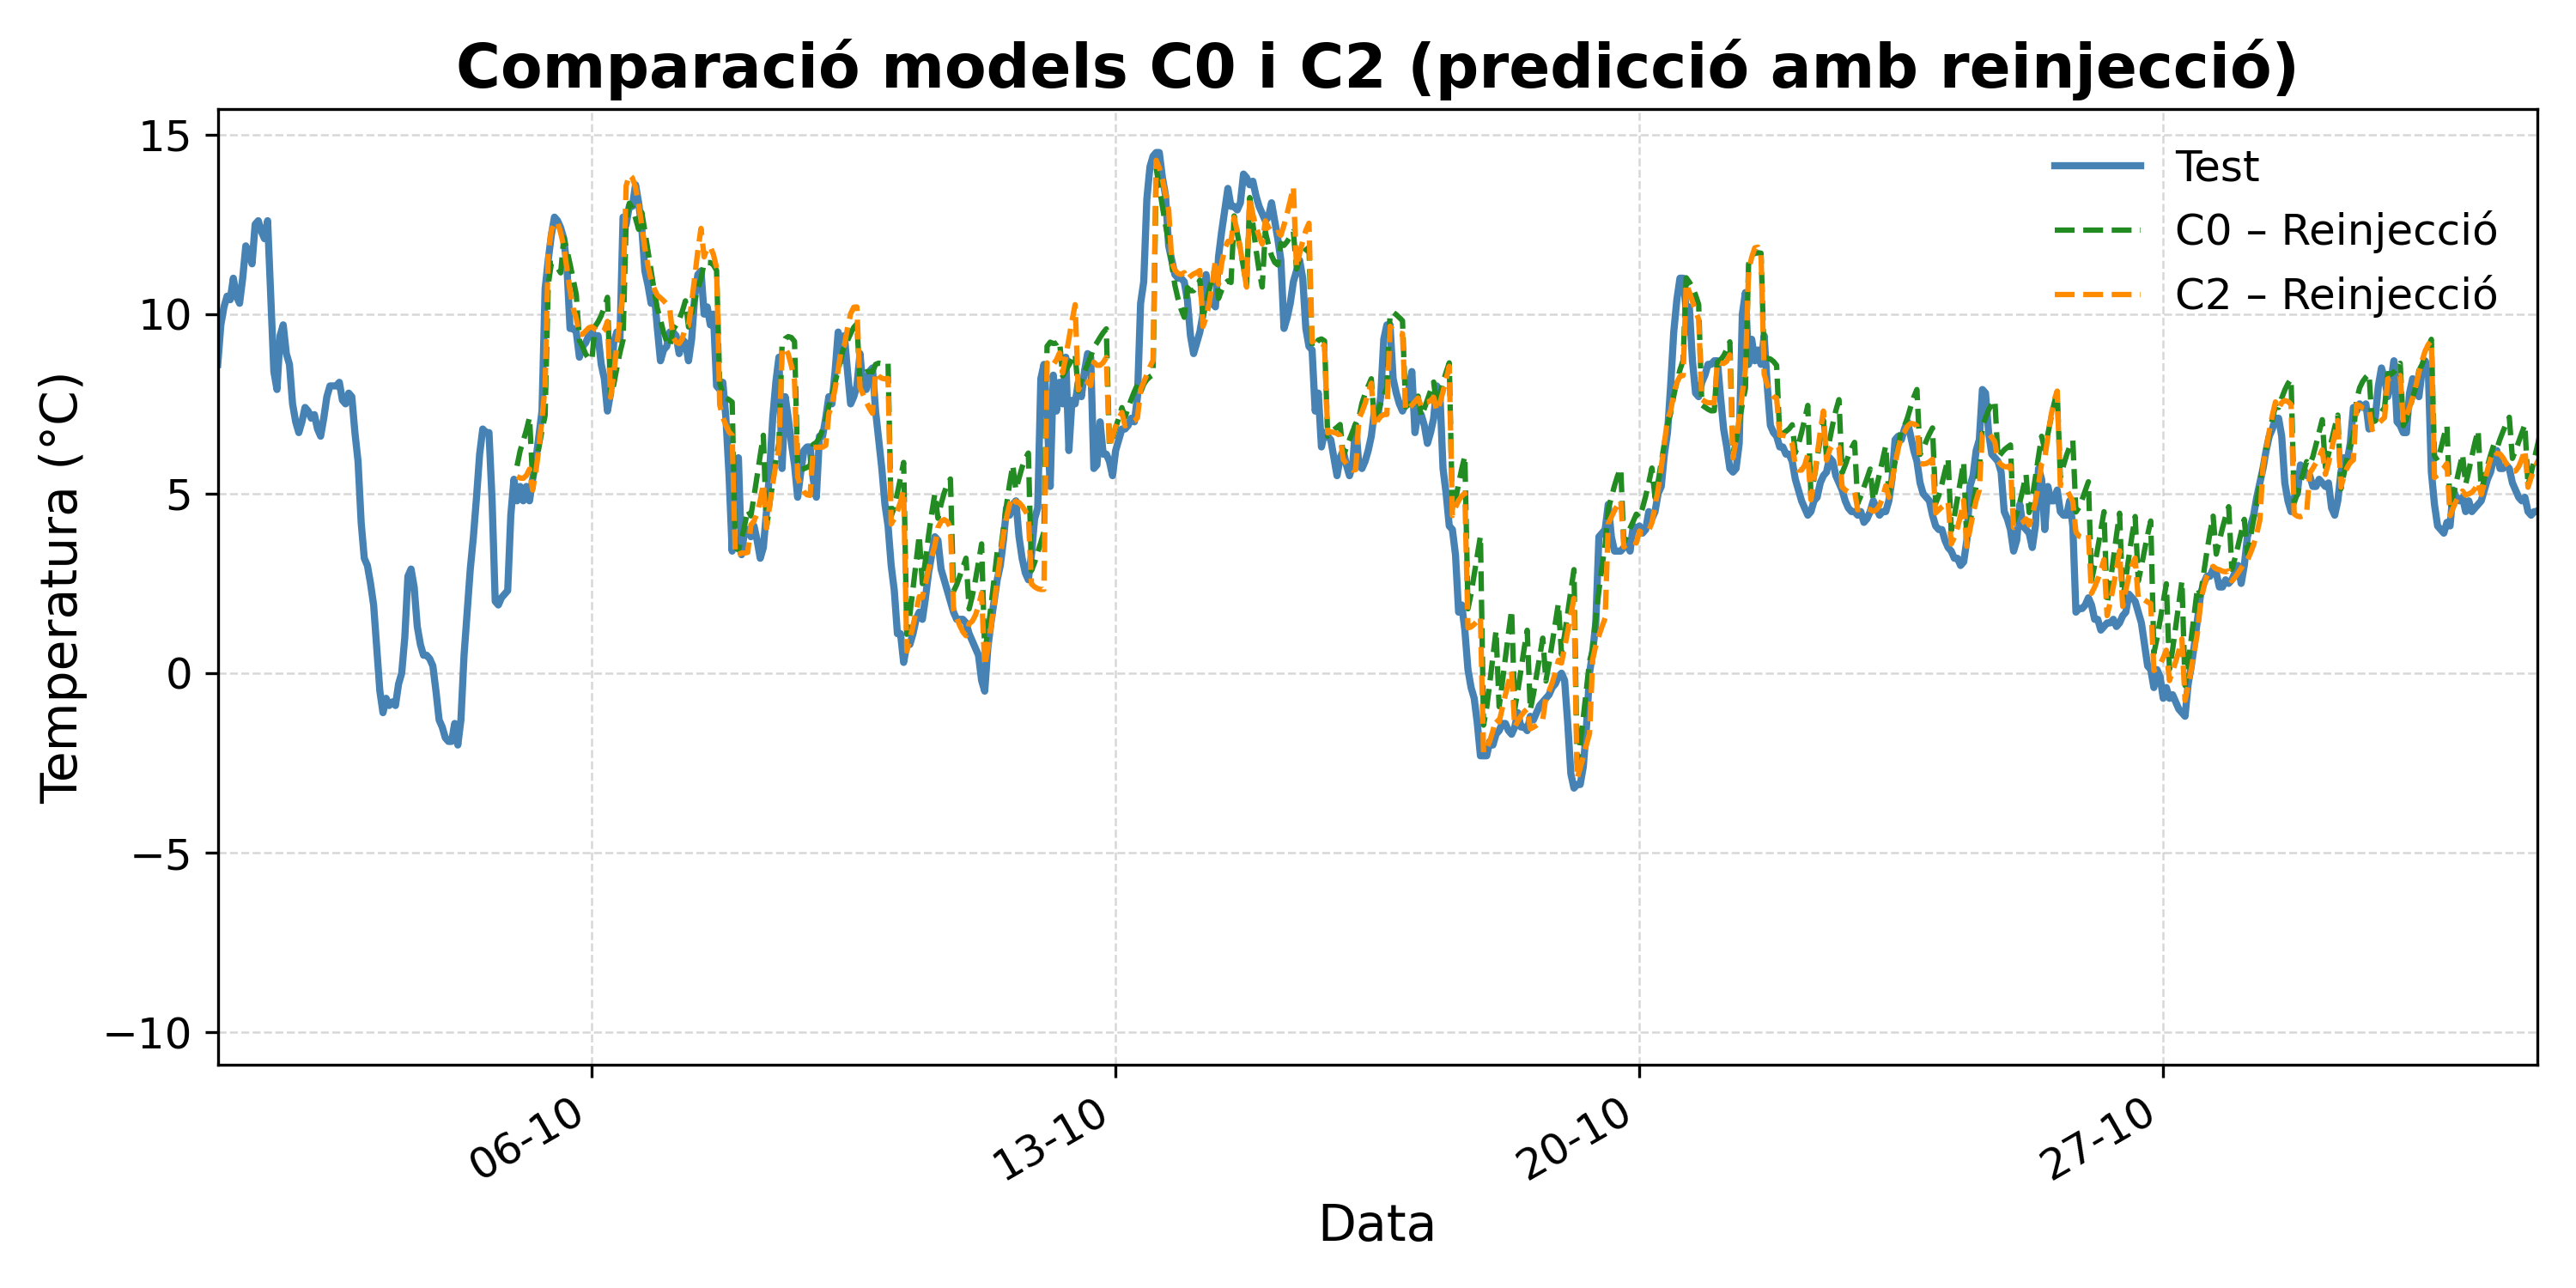
\includegraphics[width=\textwidth]{figures/lstm/results/C0_C2_plot_def.png}
        \caption{Comparació \texttt{C0} vs \texttt{C2} (reinjecció)}
        \label{fig:c0c2}
    \end{subfigure}

    \caption{Visualització de les prediccions obtingudes pels diferents models LSTM destacats.}
    \label{fig:resultats_lstm_2x2}
\end{figure}


% ------------------------------------------------------------
% Fi del document
% ------------------------------------------------------------
\end{document}
